% !TEX root = ../../seminar.tex

\subsection {Scientific Method}
\label{subsec:scientific method}

The scientific method is a model which describes the working process of scientific working in general. In figure \ref{fig:SCIENTIFIC_METHOD}, the \checklist{} process is mapped on the scientific method. The colors indicate which steps of \checklist{} correspond to which steps of the scientific process. \\
A large part of the scientific method is focused on finding research topics (white) and formulating research questions (yellow). In contrast \checklist{} focuses on answering the research question. This is represented by multiple colors being mapped onto only two steps and two transitions in figure  \ref{fig:SCIENTIFIC_METHOD}. The steps marked white are not contained in \checklist{}.
The different focuses are caused by advisors usually assigning students a narrow research topic or a specific research question.

\begin{figure}
	\centering
	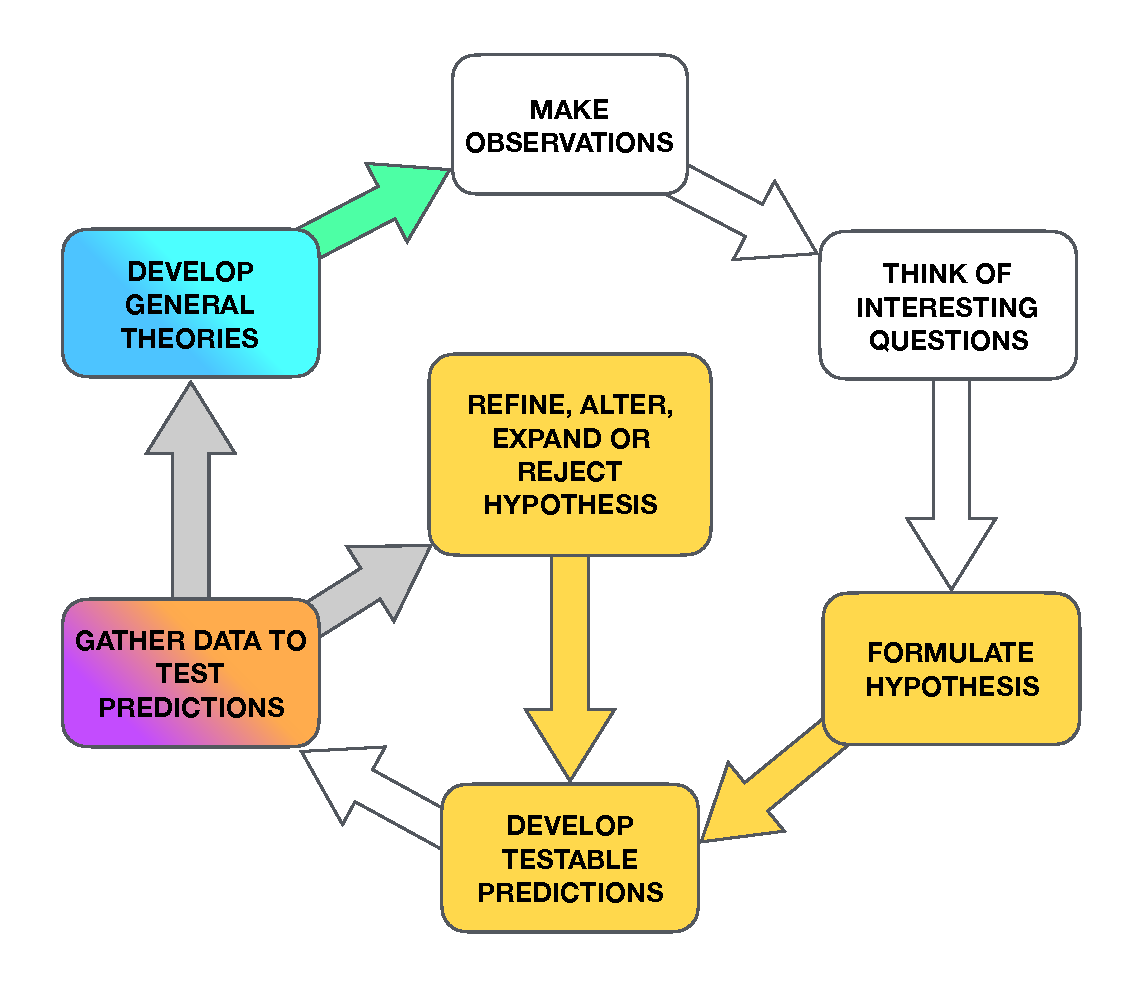
\includegraphics[width=12cm]{figures/scientific_method_mapping.pdf}
	\caption{Mapping of our process to the scientific method \cite{ScienceMethod}.}
	\label{fig:SCIENTIFIC_METHOD}
\end{figure}


